\chapter{适应性免疫与疫苗接种}\label{ch:g12:adaptive-immunity}

1796 年，一位乡村医生从一名挤奶女工的牛痘疱疹中取出脓液，
划入一名男孩的手臂，等待六周后，又对他接种天花病毒。
男孩没有发病。医生所处的时代无法解释其中缘由，
机体似乎已被“教会”了。两个世纪后，天花已经灭绝，
而如今这一机制已可在分子层面得到解释：一群\omterm{def:g10:cells-common-unit:cell}{细胞}共同携带着
几乎能识别任何可能存在的分子的受体，
在相应分子出现时增殖，
并能形成记忆。本章介绍这一系统、
其两条分支、其记忆功能、
以此为基础研制的\omterm{def:g12:adaptive-immunity:vaccine}{疫苗}，以及摧毁它的病毒。

\section{抗原与淋巴细胞}

\begin{definition}[抗原、淋巴细胞]\label{def:g12:adaptive-immunity:antigen}
\emph{抗原}\index{抗原}是指\omterm{def:g12:innate-immunity:immunity}{适应性免疫}系统能够识别的
任何分子，通常是微生物的\omterm{def:g11:gene-expression:protein}{蛋白质}或\omterm{def:g10:chemistry-of-life:families}{糖类}、
毒素、外来\omterm{def:g10:cells-common-unit:cell}{细胞}的表面，或错误地指机体自身的
某种分子。能够识别抗原的\omterm{def:g10:cells-common-unit:cell}{细胞}是
\emph{淋巴细胞}\index{淋巴细胞}，即在骨髓中产生的白\omterm{def:g10:cells-common-unit:cell}{细胞}，
聚集于淋巴结、脾和肠道的
淋巴组织中。每个淋巴\omterm{def:g10:cells-common-unit:cell}{细胞}携带数千份同一种
\emph{受体}，每种受体只结合一种抗原。
\emph{B 淋巴\omterm{def:g10:cells-common-unit:cell}{细胞}}在骨髓中成熟，并将产生\omterm{prop:g12:adaptive-immunity:antibodies}{抗体}；
\emph{T 淋巴\omterm{def:g10:cells-common-unit:cell}{细胞}}在胸腺中成熟，通过接触和
信号发挥作用。
\end{definition}

\begin{proposition}[预先生成的受体库]\label{prop:g12:adaptive-immunity:repertoire}
每个\omterm{def:g12:adaptive-immunity:antigen}{淋巴细胞}的受体在\omterm{def:g10:cells-common-unit:cell}{细胞}成熟过程中，
由\omterm{def:g10:universal-dna:gene}{基因}片段的随机重排装配而成，各\omterm{def:g10:cells-common-unit:cell}{细胞}互不相同。
因此机体在接触\omterm{def:g12:adaptive-immunity:antigen}{抗原}之前，已持有约 $10^{8}$ 种不同的受体，
足以使几乎任何分子都能找到少数能与之结合的\omterm{def:g10:cells-common-unit:cell}{细胞}。
受体能够结合机体自身分子的\omterm{def:g12:adaptive-immunity:antigen}{淋巴细胞}在成熟过程中被清除；
其余\omterm{def:g12:adaptive-immunity:antigen}{淋巴细胞}则各自等待，每种可能的\omterm{def:g12:adaptive-immunity:antigen}{抗原}对应少数\omterm{def:g10:cells-common-unit:cell}{细胞}，
直至相应\omterm{def:g12:adaptive-immunity:antigen}{抗原}出现。
\end{proposition}
\admitted

\begin{omfigure}
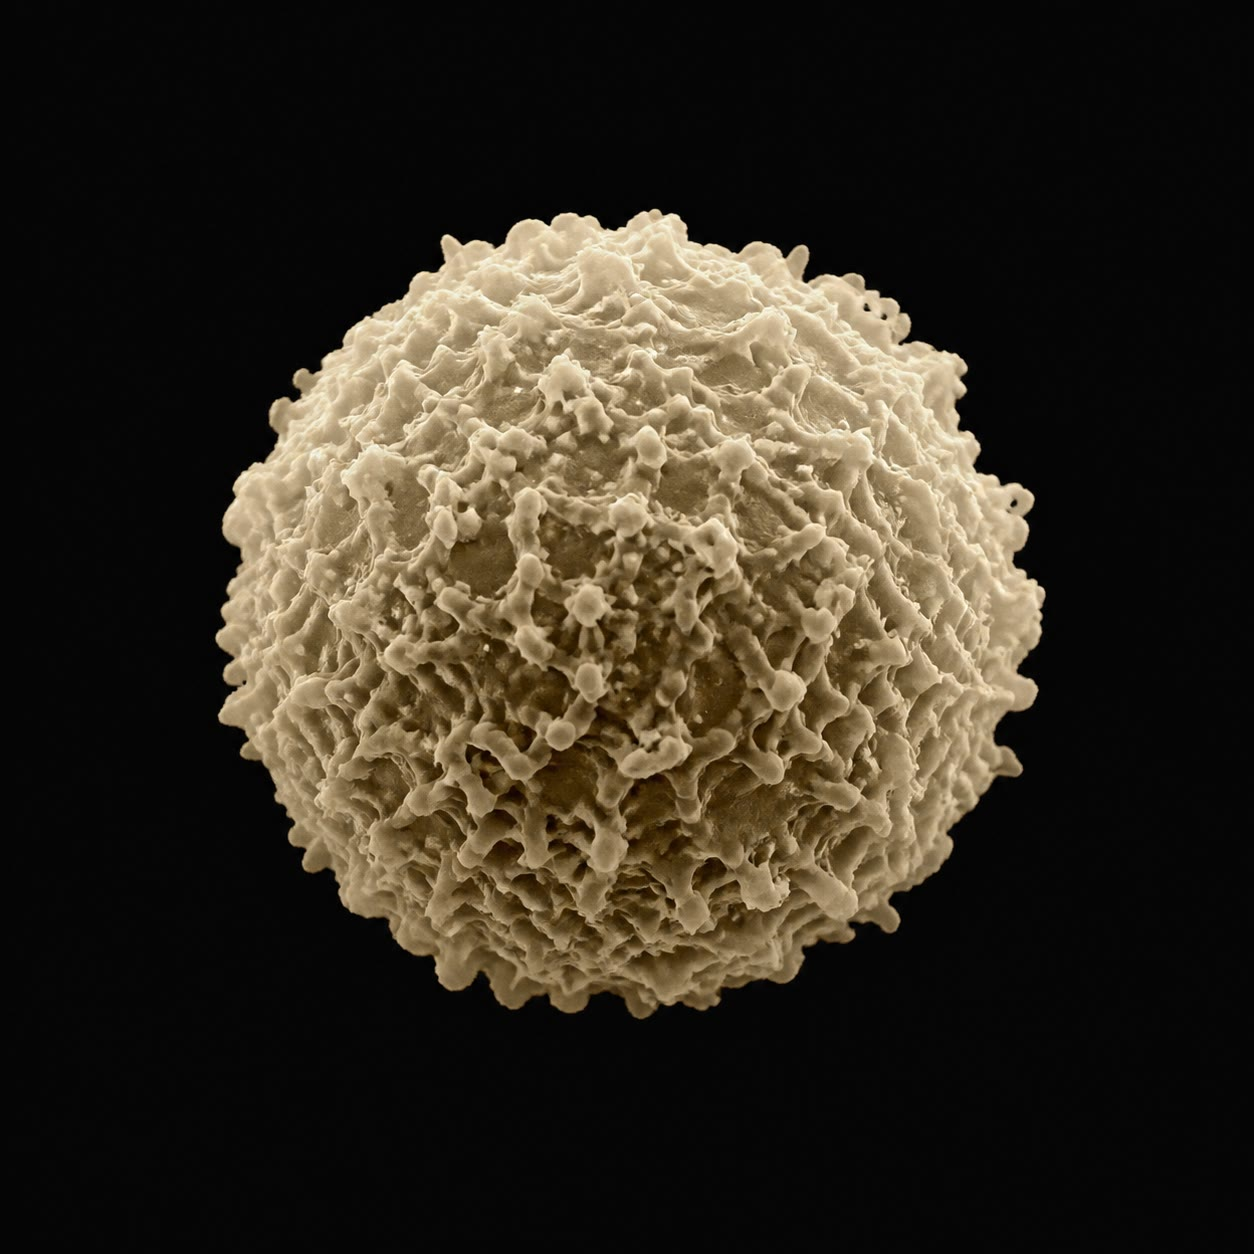
\includegraphics[width=0.36\linewidth]{images/book2/ai/g12-adaptive-lymphocyte-sem.jpg}

{\small \omterm{def:g12:adaptive-immunity:antigen}{淋巴细胞}的伪彩色电子显微照片：一个
表面粗糙的小圆形\omterm{def:g10:cells-common-unit:cell}{细胞}，属于约一亿种中的一种，
每种\omterm{def:g10:cells-common-unit:cell}{细胞}都携带针对单一\omterm{def:g12:adaptive-immunity:antigen}{抗原}的受体。}
\end{omfigure}

\section{克隆选择}

\begin{proposition}[选择与扩增]\label{prop:g12:adaptive-immunity:selection}
\omterm{def:g12:adaptive-immunity:antigen}{抗原}入侵时，只有受体与之匹配的\omterm{def:g12:adaptive-immunity:antigen}{淋巴细胞}发生应答，
它们被\emph{选择}，并通过\omterm{def:g11:cell-cycle-mitosis:cycle}{有丝分裂}在数日内增殖为
由数千个相同\omterm{def:g10:cells-common-unit:cell}{细胞}组成的克隆——
\emph{克隆选择}\index{克隆选择}。随后，克隆发生分化：
多数\omterm{def:g10:cells-common-unit:cell}{细胞}成为\emph{效应\omterm{def:g10:cells-common-unit:cell}{细胞}}，在一周或两周内对抗\omterm{def:g12:adaptive-immunity:antigen}{抗原}后死亡；
少数\omterm{def:g10:cells-common-unit:cell}{细胞}则成为长寿的
\emph{记忆细胞}\index{记忆细胞}，可存活数年；若\omterm{def:g12:adaptive-immunity:antigen}{抗原}再次出现，
它们将更快、以多得多的数量作出应答。该应答具有专一性，因为只有
匹配的克隆才会扩增；首次应答较慢，是因为它们从少量\omterm{def:g10:cells-common-unit:cell}{细胞}开始增殖；
再次应答较快，
是因为\omterm{prop:g12:adaptive-immunity:selection}{记忆细胞}已经大量存在。
\end{proposition}
\begin{proof}[证据]
针对某一\omterm{def:g12:adaptive-immunity:antigen}{抗原}的\omterm{prop:g12:adaptive-immunity:antibodies}{抗体}在首次注射后约一周出现于血液中，
持续上升两周后下降；数月后进行第二次注射，
两三天内即可产生
十至一百倍于第一次峰值的\omterm{prop:g12:adaptive-immunity:antibodies}{抗体}，并可持续数年。
若在第二次注射的同时注射另一种无关\omterm{def:g12:adaptive-immunity:antigen}{抗原}，
则该\omterm{def:g12:adaptive-immunity:antigen}{抗原}只能引发缓慢的初次应答，说明记忆具有专一性。
从已免疫动物体内取出的\omterm{def:g12:adaptive-immunity:antigen}{淋巴细胞}，
移入未免疫的动物体内即可转移其记忆；
取自未免疫动物的\omterm{def:g12:adaptive-immunity:antigen}{淋巴细胞}则不能。
\end{proof}

\begin{omfigure}
\begin{tikzpicture}[font=\small, >=Stealth]
  \tikzset{lc/.style={circle, draw, thick, fill=omDef!15, minimum size=0.55cm, inner sep=0},
           sel/.style={circle, draw, thick, fill=omThm!35, minimum size=0.55cm, inner sep=0},
           mem/.style={circle, draw, thick, fill=omMeth!35, minimum size=0.55cm, inner sep=0}}
  % repertoire
  \foreach \y in {2.4,1.6,0.8,0,-0.8,-1.6} \node[lc] at (0,\y) {};
  \node[sel] at (0,0.8) {};
  \foreach \y/\a in {2.4/90,1.6/45,0.8/0,0/-45,-0.8/135,-1.6/180} \draw[thick] (0.28,\y) -- ++(\a:0.001);
  \node[anchor=south, align=center] at (0,3.0) {受体库：每个细胞一种 \\ 受体};
  % antigen
  \node[draw, fill=omThm!60, minimum size=0.25cm, inner sep=0] (ag) at (1.6,0.8) {};
  \node[anchor=north, font=\scriptsize] at (1.6,0.6) {抗原};
  \draw[->, thick] (ag) -- (0.35,0.8);
  % expansion
  \draw[->, thick] (2.4,0.8) -- (3.6,0.8) node[midway, above, font=\scriptsize, align=center] {选择，\\ 增殖};
  \foreach \x in {4.2,4.9,5.6,6.3,7.0} \foreach \y in {1.6,0.8,0} \node[sel] at (\x,\y) {};
  \node[anchor=south, align=center] at (5.6,2.2) {相同细胞组成的克隆 \\ （数日）};
  % differentiation
  \draw[->, thick] (7.6,1.2) -- (8.8,1.8);
  \draw[->, thick] (7.6,0.4) -- (8.8,-0.2);
  \foreach \x in {9.4,10.1,10.8} \node[sel] at (\x,1.8) {};
  \node[anchor=west, align=left] at (11.2,1.8) {效应细胞：\\ 立即作战，随后死亡};
  \foreach \x in {9.4,10.1} \node[mem] at (\x,-0.2) {};
  \node[anchor=west, align=left] at (11.2,-0.2) {记忆细胞：\\ 数年待命};
\end{tikzpicture}

{\small \omterm{prop:g12:adaptive-immunity:selection}{克隆选择}。在储备的众多\omterm{def:g12:adaptive-immunity:antigen}{淋巴细胞}克隆中，
\omterm{def:g12:adaptive-immunity:antigen}{抗原}选择受体与之匹配的那一个；它
在数日内增殖为执行战斗的效应\omterm{def:g10:cells-common-unit:cell}{细胞}和
持续存在的\omterm{prop:g12:adaptive-immunity:selection}{记忆细胞}。再次相遇时，记忆克隆已然庞大。}
\end{omfigure}

\begin{omfigure}
\begin{tikzpicture}
\begin{axis}[
  width=0.9\linewidth, height=5.8cm,
  axis x line=bottom, axis y line=left,
  xmin=0, xmax=80, ymin=0, ymax=110,
  xlabel={天}, ylabel={血液中抗体（相对值）},
  xlabel style={font=\small, at={(axis description cs:0.5,-0.12)}, anchor=north},
  ylabel style={font=\small},
  tick label style={font=\small}, xtick={0,10,20,30,40,50,60,70,80}, ytick={0,25,50,75,100},
  clip=false,
]
\addplot[thick, omThm, smooth] coordinates {(0,0) (5,0) (7,1) (10,4) (14,9) (18,10) (24,8) (30,5) (40,3) (50,2) (60,20) (63,60) (66,95) (70,100) (76,92) (80,85)};
\draw[->, thick] (axis cs:1,-14) -- (axis cs:1,-2); \node[font=\scriptsize, anchor=north] at (axis cs:1,-15) {初次注射};
\draw[->, thick] (axis cs:56,-14) -- (axis cs:56,-2); \node[font=\scriptsize, anchor=north] at (axis cs:56,-15) {再次注射};
\node[font=\scriptsize, anchor=south] at (axis cs:18,12) {初次应答};
\node[font=\scriptsize, anchor=east] at (axis cs:68,100) {再次应答};
\end{axis}
\end{tikzpicture}

{\small 同一\omterm{def:g12:adaptive-immunity:antigen}{抗原}两次注射后的\omterm{prop:g12:adaptive-immunity:antibodies}{抗体}。初次
应答在一周后开始，且维持在较低水平；来自\omterm{prop:g12:adaptive-immunity:selection}{记忆细胞}的
再次应答数日内即开始，水平可达前者的十倍——
这正是加强剂量的原理。}
\end{omfigure}

\section{两条臂：抗体与杀伤细胞}

\begin{proposition}[B 淋巴细胞与抗体]\label{prop:g12:adaptive-immunity:antibodies}
被选中的 B 克隆分化为\emph{浆\omterm{def:g10:cells-common-unit:cell}{细胞}}，它们是
每秒分泌数千个\emph{抗体}\index{抗体}的“工厂”：
该克隆受体的可溶性拷贝，呈 Y 形的\omterm{def:g11:gene-expression:protein}{蛋白质}，其两臂
各自结合\omterm{def:g12:adaptive-immunity:antigen}{抗原}。\omterm{prop:g12:adaptive-immunity:antibodies}{抗体}并不直接杀伤，而是\emph{标记}。
与病毒或毒素结合后，\omterm{prop:g12:adaptive-immunity:antibodies}{抗体}可阻止它们进入\omterm{def:g10:cells-common-unit:cell}{细胞}或
发挥作用；与细菌结合后，\omterm{prop:g12:adaptive-immunity:antibodies}{抗体}将其包被，这层包被正是
\omterm{def:g12:innate-immunity:phagocytosis}{吞噬细胞}（见\cref{ch:g12:innate-immunity}）最易抓住的部分。\omterm{def:g12:adaptive-immunity:antigen}{抗原}
被多个\omterm{prop:g12:adaptive-immunity:antibodies}{抗体}交联后聚集成\emph{免疫复合物}，
再经\omterm{def:g12:innate-immunity:phagocytosis}{吞噬作用}清除。这一臂负责对付血液和体液中的
入侵者。
\end{proposition}
\admitted

\begin{omfigure}
\begin{tikzpicture}[font=\small, line cap=round, >=Stealth]
  % antibody Y
  \draw[line width=5pt, omDef!70] (0,-1.6) -- (0,0);
  \draw[line width=5pt, omDef!70] (0,0) -- (-1.1,1.3);
  \draw[line width=5pt, omDef!70] (0,0) -- (1.1,1.3);
  \draw[line width=3pt, omDef!35] (0.25,-1.6) -- (0.25,0.05) -- (1.3,1.1);
  \draw[line width=3pt, omDef!35] (-0.25,-1.6) -- (-0.25,0.05) -- (-1.3,1.1);
  \node[draw, fill=omThm!60, minimum size=0.28cm, inner sep=0, rotate=40] at (-1.35,1.6) {};
  \node[draw, fill=omThm!60, minimum size=0.28cm, inner sep=0, rotate=-40] at (1.35,1.6) {};
  \node[anchor=west, align=left] at (1.9,1.6) {抗原结合于 \\ 每条臂的末端};
  \node[anchor=west, align=left] at (1.9,-1.2) {茎：被吞噬细胞 \\ 抓住};
  \draw[->] (1.85,-1.2) -- (0.35,-1.2);
  \node[anchor=north, align=center] at (0,-1.9) {一个抗体：两条臂，\\ 一种专一性};
  % complex
  \begin{scope}[xshift=8.6cm]
    \foreach \x/\y in {0/0, 1.2/0.6, 0.4/1.3, 1.6/-0.5, -0.6/0.9}
      \node[draw, fill=omThm!60, minimum size=0.28cm, inner sep=0] at (\x,\y) {};
    \foreach \a/\b in {0/0.6, 0.6/1.15, 1.15/0.65, 0.65/1.45, 1.45/-0.05, -0.05/0.75, 0.75/-0.6}
      \draw[line width=2.5pt, omDef!70] (\a,\b) -- ++(0.35,-0.25);
    \draw[line width=2.5pt, omDef!70] (0.1,0.05) -- (1.1,0.55); \draw[line width=2.5pt, omDef!70] (0.5,1.2) -- (1.15,0.65);
    \draw[line width=2.5pt, omDef!70] (-0.5,0.85) -- (0.3,1.25); \draw[line width=2.5pt, omDef!70] (1.25,0.5) -- (1.55,-0.4);
    \draw[line width=2.5pt, omDef!70] (0.05,-0.05) -- (1.5,-0.45);
    \node[anchor=north, align=center] at (0.5,-1.4) {免疫复合物：抗原 \\ 已交联，待吞噬};
  \end{scope}
\end{tikzpicture}

{\small \omterm{prop:g12:adaptive-immunity:antibodies}{抗体}及其作用。两臂结合\omterm{def:g12:adaptive-immunity:antigen}{抗原}；
茎部被\omterm{def:g12:innate-immunity:phagocytosis}{吞噬细胞}识别。许多\omterm{prop:g12:adaptive-immunity:antibodies}{抗体}结合许多
\omterm{def:g12:adaptive-immunity:antigen}{抗原}，形成复合物，\omterm{def:g12:innate-immunity:phagocytosis}{吞噬细胞}可整体吞入。}
\end{omfigure}

\begin{proposition}[T 淋巴细胞]\label{prop:g12:adaptive-immunity:tcells}
T \omterm{def:g12:adaptive-immunity:antigen}{淋巴细胞}只能识别以片段形式
呈递于另一\omterm{def:g10:cells-common-unit:cell}{细胞}表面的\omterm{def:g12:adaptive-immunity:antigen}{抗原}（见\cref{ch:g12:innate-immunity}）。共两类：
\begin{itemize}
  \item \emph{辅助性 T 细胞}\index{辅助性 T 细胞}
        在将\omterm{def:g12:adaptive-immunity:antigen}{抗原}带至淋巴结的\omterm{prop:g12:innate-immunity:handover}{树突状细胞}作用下被激活；
        一经选择并增殖，便分泌\omterm{def:g10:cells-common-unit:cell}{细胞}因子，
        以授权并增强 B \omterm{def:g12:adaptive-immunity:antigen}{淋巴细胞}和其他
        T \omterm{def:g12:adaptive-immunity:antigen}{淋巴细胞}的应答。它们是协调者；没有它们，几乎
        不会发生适应性应答。
  \item \emph{\omterm{def:g10:cells-common-unit:cell}{细胞}毒性 T \omterm{def:g10:cells-common-unit:cell}{细胞}}识别被感染\omterm{def:g10:cells-common-unit:cell}{细胞}呈递的病毒
        （或\omterm{def:g11:cancer:cancer}{肿瘤}蛋白）片段，并通过接触杀死该\omterm{def:g10:cells-common-unit:cell}{细胞}，
        赶在其中的病毒增殖之前。
        这一臂负责对付藏匿在\omterm{def:g10:cells-common-unit:cell}{细胞}内、\omterm{prop:g12:adaptive-immunity:antibodies}{抗体}
        无法到达的入侵者。
\end{itemize}
\end{proposition}
\admitted

\begin{omfigure}
\begin{tikzpicture}[font=\small, >=Stealth,
  b/.style={draw, rounded corners, align=center, text width=2.8cm, minimum height=1.1cm}]
  \node[b, fill=omProp!15] (dc) at (0,0) {树突状细胞 \\ 呈递抗原 \\ 片段};
  \node[b, fill=omThm!15, text width=3.0cm] (th) at (4.4,0) {辅助性 T 细胞：\\ 被选择、增殖、\\ 分泌细胞因子};
  \node[b, fill=omDef!12] (bc) at (9.2,1.6) {B 淋巴细胞：浆细胞，\\ 抗体};
  \node[b, fill=omDef!12] (tc) at (9.2,-1.6) {细胞毒性 T 细胞：\\ 杀伤被感染细胞};
  \node[b, fill=omMeth!15, text width=2.4cm] (mem) at (13.2,0) {记忆细胞 \\ 三类皆有};
  \draw[->, thick] (dc) -- (th);
  \draw[->, thick] (th) -- node[above, sloped, font=\scriptsize] {细胞因子} (bc);
  \draw[->, thick] (th) -- node[below, sloped, font=\scriptsize] {细胞因子} (tc);
  \draw[->, thick] (bc) -- (mem); \draw[->, thick] (tc) -- (mem); \draw[->, thick] (th) -- (mem);
\end{tikzpicture}

{\small 适应性应答的组织方式。\omterm{prop:g12:innate-immunity:handover}{树突状
细胞}的信息激活辅助性 T \omterm{def:g10:cells-common-unit:cell}{细胞}，其\omterm{def:g10:cells-common-unit:cell}{细胞}因子
授权 B \omterm{def:g12:adaptive-immunity:antigen}{淋巴细胞}产生\omterm{prop:g12:adaptive-immunity:antibodies}{抗体}，授权\omterm{def:g10:cells-common-unit:cell}{细胞}毒性 T \omterm{def:g10:cells-common-unit:cell}{细胞}杀伤；
每条臂都会留下\omterm{prop:g12:adaptive-immunity:selection}{记忆细胞}。}
\end{omfigure}

\begin{example}[同一病毒，两次相遇]\label{ex:g12:adaptive-immunity:virus}
初次流感：病毒增殖三天后，
适应性应答才准备就绪；第 7 天时，\omterm{def:g10:cells-common-unit:cell}{细胞}毒性 T \omterm{def:g10:cells-common-unit:cell}{细胞}正在杀伤
呼吸道中的感染\omterm{def:g10:cells-common-unit:cell}{细胞}，\omterm{prop:g12:adaptive-immunity:antibodies}{抗体}正在中和游离
病毒；第 10 天时，此人正在康复，体内已有
两类\omterm{prop:g12:adaptive-immunity:selection}{记忆细胞}。一年后遇到同一毒株时，血液中已有的\omterm{prop:g12:adaptive-immunity:antibodies}{抗体}
在侵入时即阻挡大部分病毒，\omterm{prop:g12:adaptive-immunity:selection}{记忆细胞}两天内即增殖，
感染尚未被察觉便已结束。若毒株不同，其
表面蛋白发生\omterm{def:g11:mutations:mutation}{突变}，便能逃过\omterm{prop:g12:adaptive-immunity:antibodies}{抗体}——这正是
\omterm{def:g12:adaptive-immunity:vaccine}{疫苗}每年都要重新制备的原因。
\end{example}

\section{疫苗接种}

\begin{definition}[疫苗]\label{def:g12:adaptive-immunity:vaccine}
称\emph{疫苗}\index{疫苗}为一种制剂，可引发
针对某种病原体的初次适应性应答并由此产生记忆，
而不引起其所致疾病：病原体经减毒（麻疹、
结核）、灭活（注射用脊髓灰质炎疫苗），或只剩其中某一
\omterm{def:g11:gene-expression:protein}{蛋白质}或灭活毒素（破伤风、乙型肝炎），或者，最近，
改为仅含让\omterm{def:g10:cells-common-unit:cell}{细胞}合成该\omterm{def:g11:gene-expression:protein}{蛋白质}的指令。制剂中加入的
\emph{佐剂}可引发轻微炎症，
没有这种炎症，\omterm{prop:g12:innate-immunity:handover}{树突状细胞}便无法将\omterm{def:g12:adaptive-immunity:antigen}{抗原}带至淋巴结。加强剂量
可使初次应答转为再次应答，
并将记忆延长数十年。
\end{definition}

\begin{omfigure}

\includegraphics[width=0.56\linewidth]{images/book2/ai/g12-adaptive-vaccination.jpg}

{\small 接种\omterm{def:g12:adaptive-immunity:vaccine}{疫苗}：将\omterm{def:g12:adaptive-immunity:antigen}{抗原}注入手臂，并加入佐剂，
以引起局部炎症。数周之内，淋巴结中已储存
针对此人从未患过的疾病的\omterm{prop:g12:adaptive-immunity:selection}{记忆细胞}。}
\end{omfigure}

\begin{omfigure}
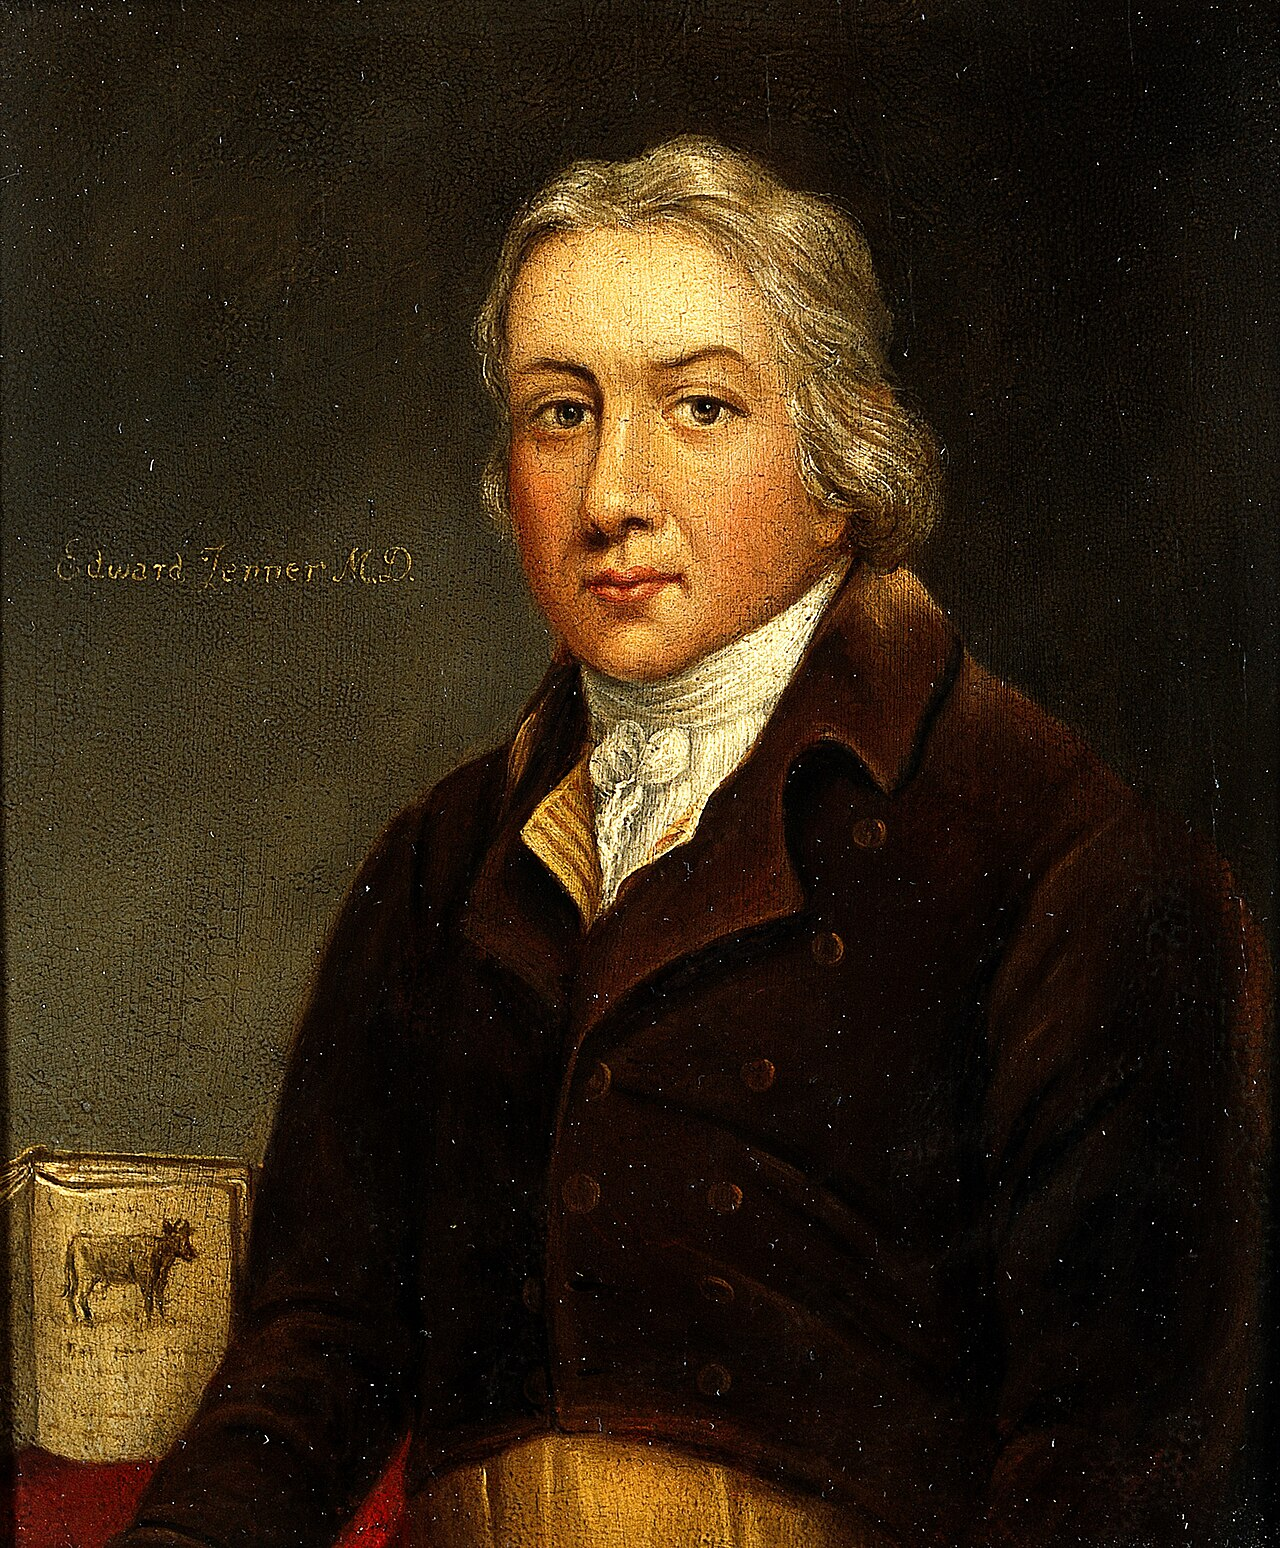
\includegraphics[width=0.34\linewidth]{images/book1/jenner.jpg}

{\small 爱德华·詹纳于 1796 年证明，接种牛痘
可预防天花——这便是\omterm{def:g12:adaptive-immunity:vaccine}{疫苗}接种，其机制当时尚未为人所知。
油画：Wellcome Collection，CC BY 4.0。}
\end{omfigure}

\begin{proposition}[群体保护]\label{prop:g12:adaptive-immunity:herd}
接种\omterm{def:g12:adaptive-immunity:vaccine}{疫苗}的个体受到保护；接种\omterm{def:g12:adaptive-immunity:vaccine}{疫苗}的人口
也能保护其中未接种的成员。感染者平均
会将疾病传给无免疫力人口中的 $R_0$ 人（麻疹约 15，
流感为 2 至 3）；若比例为 $v$ 的人已获免疫，则只有
这些接触中，$R_0(1 - v)$ 次可能感染，疾病
在该数值低于 1 时消退——即当
\[
v > 1 - \frac{1}{R_0}.
\]
麻疹需 93\% 的人口获得免疫，才能保护
年龄太小、尚不能接种\omterm{def:g12:adaptive-immunity:vaccine}{疫苗}的婴儿，以及无法接种者，
流感约需 60\%。这种\emph{群体免疫}\index{群体免疫}
正是接种\omterm{def:g12:adaptive-immunity:vaccine}{疫苗}具有集体性的原因。
\end{proposition}
\admitted

\begin{omfigure}
\begin{tikzpicture}
\begin{axis}[
  width=0.84\linewidth, height=5.4cm,
  axis x line=bottom, axis y line=left,
  xmin=0, xmax=20, ymin=0, ymax=100,
  xlabel={疾病的 $R_0$}, ylabel={所需接种比例（\%）},
  xlabel style={font=\small, at={(axis description cs:0.5,-0.12)}, anchor=north},
  ylabel style={font=\small},
  tick label style={font=\small}, xtick={0,5,10,15,20}, ytick={0,25,50,75,100},
  clip=false,
]
\addplot[thick, omThm, domain=1:20, samples=100] {100*(1-1/x)};
\draw[dashed, gray] (axis cs:2.5,0) -- (axis cs:2.5,60); \node[font=\scriptsize, anchor=west] at (axis cs:2.9,48) {流感};
\draw[dashed, gray] (axis cs:6,0) -- (axis cs:6,83); \node[font=\scriptsize, anchor=south] at (axis cs:6,85) {脊髓灰质炎};
\draw[dashed, gray] (axis cs:15,0) -- (axis cs:15,93); \node[font=\scriptsize, anchor=south] at (axis cs:15,95) {麻疹};
\end{axis}
\end{tikzpicture}

{\small 为阻止疾病传播，\omterm{def:g12:selection-drift-speciation:population}{种群}中必须具有免疫力的
个体比例，随该疾病的 $R_0$ 变化。疾病的传染性越强，
则所需的接种覆盖率越接近全体。}
\end{omfigure}

\section{协调者被摧毁时}

\begin{proposition}[HIV 与艾滋病]\label{prop:g12:adaptive-immunity:hiv}
人类免疫缺陷病毒（HIV）感染辅助性 T \omterm{def:g10:cells-common-unit:cell}{细胞}，
借由标记这些\omterm{def:g10:cells-common-unit:cell}{细胞}的那一受体侵入，并在其中
增殖。多年间，\omterm{def:g12:innate-immunity:immunity}{免疫系统}清除被感染\omterm{def:g10:cells-common-unit:cell}{细胞}，并产生
\omterm{prop:g12:adaptive-immunity:antibodies}{抗体}——患者此时为\emph{血清阳性}，且具有传染性——
而病毒不断变异，逃避每一次应答，并逐渐
耗尽辅助性 T \omterm{def:g10:cells-common-unit:cell}{细胞}。当其数量降至约为正常值的五分之一以下时，
适应性应答便无法再得到协调：
\emph{艾滋病}\index{艾滋病}阶段，原本健康人体可不知不觉清除的感染，
如口腔真菌感染、肺部的轻度寄生虫感染——
变得致命，并出现罕见\omterm{def:g11:cancer:cancer}{癌症}。抗病毒药物
可抑制病毒的酶，恢复辅助性 T \omterm{def:g10:cells-common-unit:cell}{细胞}，长期服用时
可控制病情并阻断传播；目前尚无\omterm{def:g12:adaptive-immunity:vaccine}{疫苗}，
也无治愈方法。
\end{proposition}
\admitted

\begin{omfigure}
\begin{tikzpicture}
\begin{axis}[
  width=0.9\linewidth, height=6cm,
  axis x line=bottom, axis y line=left,
  xmin=0, xmax=11, ymin=0, ymax=1200,
  xlabel={感染后的年数（未治疗）}, ylabel={每 \unit{\micro L} 血液中的辅助性 T 细胞数},
  xlabel style={font=\small, at={(axis description cs:0.5,-0.12)}, anchor=north},
  ylabel style={font=\small},
  tick label style={font=\small}, xtick={0,2,4,6,8,10}, ytick={0,200,400,600,800,1000},
  clip=false,
]
\addplot[thick, omDef, smooth] coordinates {(0,1000) (0.2,550) (0.5,800) (1,750) (3,650) (5,520) (7,380) (8,280) (9,180) (10,90) (11,40)};
\addplot[thick, omThm, dashed, smooth] coordinates {(0,50) (0.15,900) (0.4,300) (1,150) (3,170) (5,220) (7,320) (8,450) (9,650) (10,900) (11,1100)};
\draw[dashed, gray] (axis cs:0,200) -- (axis cs:11,200);
\node[font=\scriptsize, gray, anchor=north] at (axis cs:5.5,190) {艾滋病阈值};
\node[font=\scriptsize, omDef, anchor=south] at (axis cs:4,680) {辅助性 T 细胞};
\node[font=\scriptsize, omThm, anchor=north] at (axis cs:2.4,130) {血液中的病毒（相对值）};
\end{axis}
\end{tikzpicture}

{\small 未经治疗的 HIV 感染进程（取整平均值）。
病毒首次爆发后，数年间免疫应答将其压制，
而辅助性 T \omterm{def:g10:cells-common-unit:cell}{细胞}持续下降；低于每微升约 200
个时，免疫应答崩溃，病毒数量激增，
机会性感染随之出现。}
\end{omfigure}

\begin{omfigure}
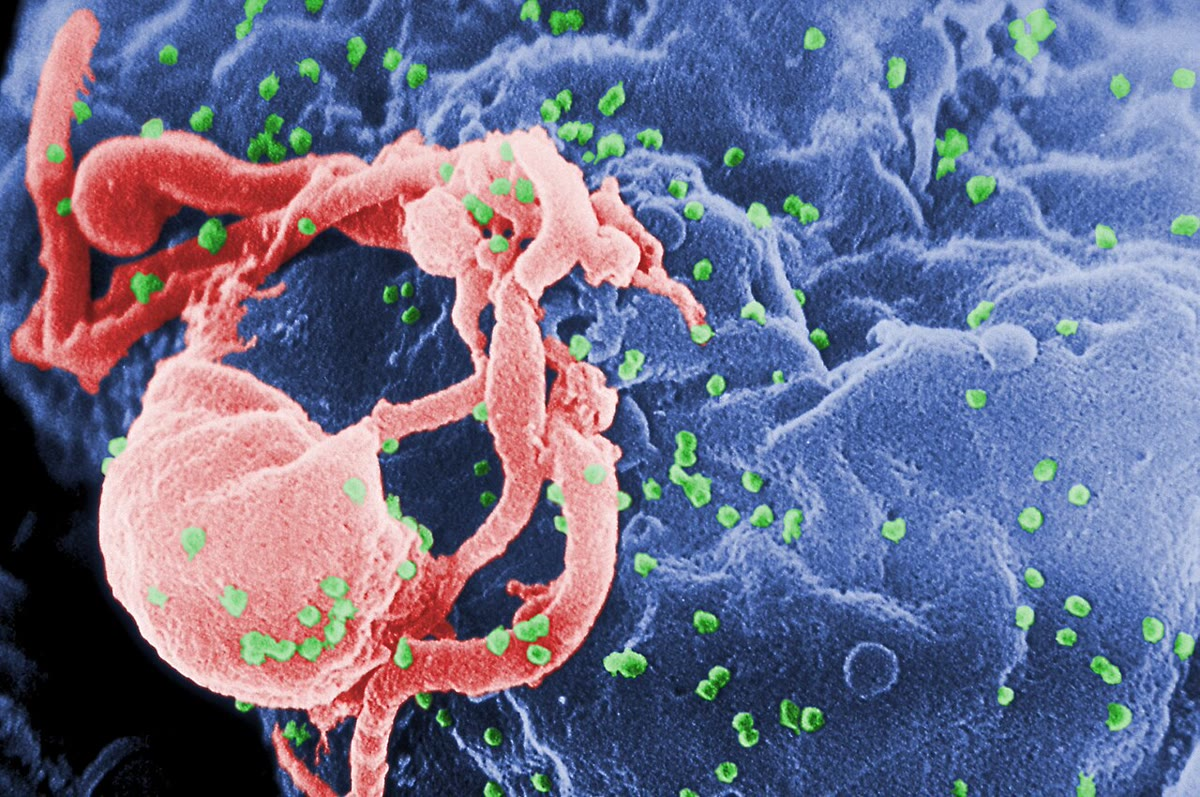
\includegraphics[width=0.6\linewidth]{images/book2/hiv-budding.jpg}

{\small 感染\omterm{def:g12:adaptive-immunity:antigen}{淋巴细胞}表面出芽的 HIV 颗粒（绿色），为假彩色电子显微照片。每个颗粒携带病毒\omterm{def:g10:universal-dna:gene}{基因}组的拷贝，其中包括下一轮应答无法识别的\omterm{def:g11:mutations:mutation}{突变}体。显微照片：C.~Goldsmith，CDC，公有领域。}
\end{omfigure}

\begin{method}[阅读免疫应答]\label{met:g12:adaptive-immunity:read}
\begin{enumerate}
  \item 确定\omterm{def:g12:adaptive-immunity:antigen}{抗原}及其所在位置：游离于体液中
        （\omterm{prop:g12:adaptive-immunity:antibodies}{抗体}起作用）或位于\omterm{def:g10:cells-common-unit:cell}{细胞}内（\omterm{def:g10:cells-common-unit:cell}{细胞}毒性 T \omterm{def:g10:cells-common-unit:cell}{细胞}起作用）。
  \item 看时间：一周左右达到峰值为初次应答，
        数天即应答则为记忆应答。
  \item 看专一性：针对一种\omterm{def:g12:adaptive-immunity:antigen}{抗原}的应答，
        不影响针对另一种\omterm{def:g12:adaptive-immunity:antigen}{抗原}的应答。
  \item 找出辅助性 T \omterm{def:g10:cells-common-unit:cell}{细胞}：没有它们，任何应答都不会发生，
        这正是\omterm{prop:g12:adaptive-immunity:hiv}{艾滋病}所说明的。
  \item 对于\omterm{def:g12:adaptive-immunity:vaccine}{疫苗}，说明\omterm{def:g12:adaptive-immunity:antigen}{抗原}的形式、佐剂、
        接种剂次数，以及所需接种的人口比例。
\end{enumerate}
\end{method}

\begin{remark}[再谈选择]\label{rem:g12:adaptive-immunity:selection}
\omterm{def:g12:innate-immunity:immunity}{适应性免疫}系统是达尔文式的：一群受体随机的\omterm{def:g10:cells-common-unit:cell}{细胞}，
其中由环境——即\omterm{def:g12:adaptive-immunity:antigen}{抗原}——挑选少数\omterm{def:g10:cells-common-unit:cell}{细胞}使其增殖，
其后代继承胜出的受体。
它在一个机体内、一周之内重演\cref{ch:g12:selection-drift-speciation}中的过程，
并借记忆将结果保留一生。
正因如此，\omterm{def:g12:innate-immunity:immunity}{免疫系统}可以被“训练”，这正是\omterm{def:g12:adaptive-immunity:vaccine}{疫苗}的作用，并解释了
为何变异快于系统选择速度的病毒——HIV、流感病毒——
如此难以战胜。
\end{remark}

\section{练习}

\begin{exercise}[$\star$]\label{exo:g12:adaptive-immunity:1}
定义\omterm{def:g12:adaptive-immunity:antigen}{抗原}和\omterm{def:g12:adaptive-immunity:antigen}{淋巴细胞}，
并说明是什么使每个\omterm{def:g12:adaptive-immunity:antigen}{淋巴细胞}具有专一性。
\end{exercise}

\begin{exercise}[$\star$]\label{exo:g12:adaptive-immunity:2}
用四个步骤描述\omterm{prop:g12:adaptive-immunity:selection}{克隆选择}。
\end{exercise}

\begin{exercise}[$\star$]\label{exo:g12:adaptive-immunity:3}
\omterm{prop:g12:adaptive-immunity:antibodies}{抗体}是什么，它与什么结合，
以及它对细菌起什么作用？
\end{exercise}

\begin{exercise}[$\star$]\label{exo:g12:adaptive-immunity:4}
说明辅助性 T \omterm{def:g10:cells-common-unit:cell}{细胞}与\omterm{def:g10:cells-common-unit:cell}{细胞}毒性 T \omterm{def:g10:cells-common-unit:cell}{细胞}的作用。
\end{exercise}

\begin{exercise}[$\star$]\label{exo:g12:adaptive-immunity:5}
\omterm{def:g12:adaptive-immunity:vaccine}{疫苗}中含有什么？它为何有效？
\end{exercise}

\begin{exercise}[$\star\star$]\label{exo:g12:adaptive-immunity:6}
根据\omterm{prop:g12:adaptive-immunity:antibodies}{抗体}图，比较初次应答与再次应答的
延迟、峰值和时长。
\end{exercise}

\begin{exercise}[$\star\star$]\label{exo:g12:adaptive-immunity:7}
第二次注射\omterm{def:g12:adaptive-immunity:antigen}{抗原} A 与第一次注射\omterm{def:g12:adaptive-immunity:antigen}{抗原} B 同时进行，
对 A 产生强而快的应答，对 B 产生弱而慢的应答。
这说明了什么？
\end{exercise}

\begin{exercise}[$\star\star$]\label{exo:g12:adaptive-immunity:8}
为何病毒一旦进入\omterm{def:g10:cells-common-unit:cell}{细胞}，\omterm{prop:g12:adaptive-immunity:antibodies}{抗体}便无法将其清除，
哪类\omterm{def:g10:cells-common-unit:cell}{细胞}可以做到？
\end{exercise}

\begin{exercise}[$\star\star$]\label{exo:g12:adaptive-immunity:9}
计算 $R_0 = 4$ 的疾病所需的\omterm{def:g12:adaptive-immunity:vaccine}{疫苗}接种覆盖度，
以及 $R_0 = 18$ 的疾病所需的覆盖度。
\end{exercise}

\begin{exercise}[$\star\star$]\label{exo:g12:adaptive-immunity:10}
为何麻疹\omterm{def:g12:adaptive-immunity:vaccine}{疫苗}接种活动能保护
年龄太小而无法接种\omterm{def:g12:adaptive-immunity:vaccine}{疫苗}的婴儿？
\end{exercise}

\begin{exercise}[$\star\star$]\label{exo:g12:adaptive-immunity:11}
根据 HIV 图，读出第 1、5 和 9 年时的辅助性 T \omterm{def:g10:cells-common-unit:cell}{细胞}数量，
并说明\omterm{prop:g12:adaptive-immunity:hiv}{艾滋病}何时开始发病。
\end{exercise}

\begin{exercise}[$\star\star\star$]\label{exo:g12:adaptive-immunity:12}
解释仅破坏辅助性 T \omterm{def:g10:cells-common-unit:cell}{细胞}，为何同时使
体液免疫与\omterm{def:g10:cells-common-unit:cell}{细胞}免疫都无法发挥作用，并结合组织图说明。
\end{exercise}

\begin{exercise}[$\star\star\star$]\label{exo:g12:adaptive-immunity:13}
血清呈阳性者体内带有抗 HIV 的\omterm{prop:g12:adaptive-immunity:antibodies}{抗体}，却
仍未获得保护。结合病毒的\omterm{def:g11:mutations:mutation}{突变}率和靶点说明原因。
\end{exercise}

\begin{exercise}[$\star\star\star$]\label{exo:g12:adaptive-immunity:14}
流感\omterm{def:g12:adaptive-immunity:vaccine}{疫苗}每年都要重新制备，而 1970 年的麻疹\omterm{def:g12:adaptive-immunity:vaccine}{疫苗}
至今仍然有效。结合病毒表面蛋白的\omterm{def:g11:mutations:mutation}{突变}，
以及记忆的专一性，说明其差异。
\end{exercise}

\begin{exercise}[$\star\star\star$]\label{exo:g12:adaptive-immunity:15}
比较\omterm{def:g12:innate-immunity:immunity}{适应性免疫}应答与\omterm{def:g12:selection-drift-speciation:population}{种群}中的\omterm{def:g12:selection-drift-speciation:selection}{自然选择}：
变异的是什么、选择的是什么、可遗传的是什么，以及
时间尺度有何不同。这一类比在何处失效？
\end{exercise}

\section{问题：百分之九十三}

\begin{problem}[{周末问题——对一次疫苗接种活动的估算：
两剂接种后的应答、群体免疫的计算、一次
麻疹暴发的建模，以及使免疫系统失效的病毒}]
\label{pb:g12:adaptive-immunity:1}
麻疹的 $R_0 = 15$。某镇有 50\,000 人，其中 90\% 的
人口已通过接种\omterm{def:g12:adaptive-immunity:vaccine}{疫苗}或既往感染获得免疫；另有 1500 人为
未满一岁的婴儿，太小而不能接种\omterm{def:g12:adaptive-immunity:vaccine}{疫苗}。

\medskip
\noindent\textbf{第一部分——个体的应答。}
一名儿童在 12 个月时接种第一剂，18 个月时接种第二剂。
\begin{enumerate}
  \item 描述第一剂之后的\omterm{prop:g12:adaptive-immunity:antibodies}{抗体}曲线：延迟、峰值、
        下降。
  \item 描述第二剂之后的\omterm{prop:g12:adaptive-immunity:antibodies}{抗体}曲线，并
        用\omterm{prop:g12:adaptive-immunity:selection}{克隆选择}解释两者的差异。
  \item \omterm{def:g12:adaptive-immunity:vaccine}{疫苗}病毒经过减毒但仍是活的，为何要用活病毒，
        它训练的是免疫应答的哪一分支，而灭活病毒
        则训练不到？
  \item 十年后，该儿童接触麻疹病毒。前三天
        会发生什么，她为何不发病？
  \item 她未接种\omterm{def:g12:adaptive-immunity:vaccine}{疫苗}的表兄接触同一病毒，描述他
        最初十天的情况，以及此后他保留了什么。
\end{enumerate}

\medskip
\noindent\textbf{第二部分——阈值。}
\begin{enumerate}[resume]
  \item 计算为使麻疹停止传播，人口中必须免疫的
        比例。
  \item 若免疫率为 90\%，一名感染者平均可感染
        多少人？该镇是否受到保护？
  \item 镇上有多少人未获免疫，其中有多少
        为婴儿？
  \item 若接种覆盖率升至 95\%，将剩余多少
        易感者？一例病例平均将再感染多少人？
  \item 用一句话解释，婴儿的安全为何取决于
        成人的决定。
\end{enumerate}

\medskip
\noindent\textbf{第三部分——一次暴发。}
一名旅行者将麻疹带入免疫率为 90\% 的该镇。
\begin{enumerate}[resume]
  \item 设每例病例感染 $15 \times 0.10 = 1.5$ 人，按
        每代间隔 12 天依次推算。第三代中有多少病例？
        第六代呢？
  \item 经过六代后，病例总数是多少？
  \item 在 5000 名易感者中，30\% 为婴儿。估算
        若病例在易感者中均匀分布，六代后病例中
        婴儿的人数。
  \item 每一代病例都会留下获得免疫的幸存者。解释
        为何暴发会自行减缓，并大致说明何时减缓。
  \item 对免疫率为 95\% 的城镇重复第 11 题，比较
        两座城镇。
\end{enumerate}

\medskip
\noindent\textbf{第四部分——系统的失效。}
一名感染 HIV 且未经治疗的患者，其辅助性 T \omterm{def:g10:cells-common-unit:cell}{细胞}
由每微升 1000 个降至 200 个，历时 8 年。
\begin{enumerate}[resume]
  \item 计算每年和每月的平均减少量。
  \item 当降至每微升 200 个时，\omterm{prop:g12:adaptive-immunity:hiv}{艾滋病}开始发生。结合
        组织示意图，解释为何\omterm{prop:g12:adaptive-immunity:antibodies}{抗体}和\omterm{def:g10:cells-common-unit:cell}{细胞}毒性 T \omterm{def:g10:cells-common-unit:cell}{细胞}都会受到影响，
        尽管只有辅助性 T \omterm{def:g10:cells-common-unit:cell}{细胞}被感染。
  \item 该患者的麻疹\omterm{prop:g12:adaptive-immunity:selection}{记忆细胞}完好。此时再接触麻疹病毒
        是否危险？请解释。
  \item 第 8 年开始抗病毒治疗，使该计数在两年内
        回升至 600 个。这说明\omterm{prop:g12:adaptive-immunity:selection}{记忆细胞}与受体库的
        情况如何，为何治疗必须持续进行？
  \item 归纳结果：保护该镇婴儿所需的覆盖率、
        一名旅行者在 90\% 免疫率下六代内引发的病例数，
        以及一旦丧失便会使整个\omterm{def:g12:innate-immunity:immunity}{适应性免疫}系统
        瓦解的那一种\omterm{def:g10:cells-common-unit:cell}{细胞}。
\end{enumerate}
\end{problem}
